
\chapter{Theory}
The purpose of this chapter is to explain the mathematical concepts behind the numerical models used in this project, and to provide useful insight in the working concepts of the algorithms developed. 

In this project the following formulations will be used. Scalar values will be non bold characters such as $d$. Vectors will be represented by bold characters $ \mathbf{x} $. Single values in a vector may be indexed using a subscript $ \mathbf{x}_i $, as in this example where the $i$'th element of $\mathbf{x}$ is represented. Vectors of higher dimension will be indexed with as many variables as dimensions. By example a single value from a three dimensional vector may accessed as $\mathbf{g}_{n,s,t}$. 


\fxnote{Write how the math is formulated}

\section{Mathematical formulation}\label{sec:OptimizationProblem}


The optimization problem at hand is a simplified energy economic model of Europe, build with focus on exploring the composition of VRES (variable renewable energy sources) on a global and national scale. In the model each country is represented as a note connected to the surrounding countries through a link. Each country has three energy producing technologies available, gas, wind and solar power. A data resolution of 1 hour is used, and simulations run over an entire year. 

Following the naming convention from \cite{PyPSA_euro_30_model}, indexing the notes in the network with the variable $n$, the power generating technologies by $s$, the hours in the year by $t$ and the possible connecting power lines by $l$, the contributing variables to the objective function describing the total annualized system cost is the following: 

\begin{itemize}
	\item Hourly dispatch of energy from the given plants in the given countries $\mathbf{g}_{n,s,t}$ with the marginal cost $\mathbf{o}_{n,s}$.
	\item Total installed capacity of the given technologies in the given countries $\mathbf{G}_{n,s}$ with the capital cost $\mathbf{c}_{n,s}$.
	\item Total installed transmission capacity for all lines $\mathbf{F}_{l}$ with the fixed annualized cost $\mathbf{c}_{l}$.
	
\end{itemize}

The objective function for the optimization problem then becomes: 

\begin{equation}
min \; p(\mathbf{x}) = \left( \sum_{n,s} \mathbf{c}_{n,s} \mathbf{G}_{n,s} + \sum_l \mathbf{c}_l \mathbf{F}_l + \sum_{n,s,t} \mathbf{o}_{n,s} \mathbf{g}_{n,s,t} \right)
\end{equation}{}

This objective function is subject to a range of constraints ensuring realistic behavior of the system. As described in \cite{PyPSA_euro_30_model} a power balance constraint is issued to ensure stable operation of the network. These constraints force the sum of energy produced and consumed in every hour to equal zero. The hourly electricity demand at each node is described by $\mathbf{d}_{n,t}$, the incidence matrix describing the line connections is given by $\mathbf{K}_{n,l}$ and the hourly transmission in each line is described as $\mathbf{f}_{l,t}$. Then the power balance constraint becomes:

\begin{equation}
\sum_s \mathbf{g}_{n,s,t} - \mathbf{d}_{n,t} = \sum_l \mathbf{K}_{n,l} \mathbf{f}_{l,t} \; \forall n,t
\end{equation}

For all conventional generators the maximum hourly dispatch of energy is limited by the installed capacity. It is important to node that for all simulations performed in this project the installed capacity is a variable. 

\begin{equation}
0\leq \mathbf{g}_{n,s,t} \leq \mathbf{G}_{n,s} \; \forall n,s,t
\end{equation}

The dispatch of variable renewable energy sources (wind and solar) is not only limited by the installed capacity, as availability, hence the name, is variable. Therefore the constraint for dispatch of variable renewable energy sources become:

\begin{equation}
0 \leq \mathbf{g}_{n,s,t} \leq \mathbf{\overline{g}}_{n,s,t} \mathbf{G}_{n,s} \; \forall n,s,t
\end{equation}

Where $\mathbf{\overline{g}_{n,s,t}}$ represents the normalized availability per unit capacity. 

The installed capacity is constrained by the geographical potential calculated in \cite{PyPSA_euro_30_model}.

\begin{equation}
0 \leq \mathbf{G}_{n,s} \leq \mathbf{G}_{n,s}^{max} \; \forall n,s
\end{equation}

All transmission lines in the model modelled with a controllable dispatch constrained by the fact that there must be energy conservation at each node the line is connected to. !! Something here about which lines is included !!!! . Furthermore the transmission in each line is limited by the installed transmission capacity in each line. 

\begin{equation}
|\mathbf{f}_{l,t}| \leq \mathbf{F}_l \; \forall l,t
\end{equation}

In the model it is possible to activate a CO2 constraint, limiting the allowed CO2 emissions for the entire energy network. As in \cite{PyPSA_euro_30_model} the constraint is implemented using the specific emissions $\mathbf{e}_s$ in CO2-tonne-per-MWh of the fuel for each generator type $s$, with the efficiency $\mathbf{\eta}_s$ and the CO2 limit $CAP_{CO_2}$. 

\begin{equation}
\sum_{n,s,t} \frac{1}{\mathbf{\eta}_s}\mathbf{g}_{n,s,t} \mathbf{e}_s \leq CAP_{CO_2}
\end{equation}

The model is implemented in the open source software PyPSA \cite{Pypsa}, using much of the software presented in \cite{PyPSA_euro_30_model}. Optimization of the model is performed with the optimization software Gurobi \cite{Gurobi}. 

In broader terms the problem can be formulated as 

\begin{equation}
	\begin{split}
	minimize \;&\; f_0(\mathbf{x})   \; \\
	subject \; to \; &\; \mathbf{f}_i(\mathbf{x}) \leq 0 \; \; i=1..m\\
		\;			&\;  \mathbf{h}_i(\mathbf{x}) = 0 \; \; i=1..p\\
	\end{split}
\end{equation}

Where all constraints are collected in the vector functions  $\mathbf{f}_i$ and $\mathbf{h}_i$, and are rewritten to be either less than or equal to $0$. 

\section{Properties of the near optimal feasible space}\label{sec:properties_of_hull}

Analyzing the original optimization problem one can deduct that the set including all feasible solutions $W$, given by equation \ref{eq:feasible_space}, must be convex, as all constraints $f_i$ and the objective function $f_0$, are linear and therefore satisfy equation \vref{eq:convex_requirement}, thus ensuring convexity \cite{ConvexOpimization}. 

\begin{equation}\label{eq:convex_requirement}
f_i(\alpha x + \beta y) \leq \alpha f_i(x) + \beta f_i(y) \; \forall \; x, y \in \mathbb{R}^d and  \; \alpha, \beta \in \mathbb{R}
\end{equation}

Furthermore, when all variables are bounded; hourly production by the power balance constraint and installed capacity by geographical potential and CO2 emission constraints, the feasible decision space is not only convex but also closed. If the geographical potential constraint, or the CO2 emission limit is excluded the feasible decision space becomes an open convex space as illustrated on \vref{fig:sketch_feasable_space}, this does however not have any immediate consequences, as the objective function increases as one moves in the open direction of the space. 

\begin{figure}[ht]
	\centering
	\incfig{Feasible-space}
	\caption{A sketch of a one dimensional feasible space with MGA constraint }
	\label{fig:sketch_feasable_space}
\end{figure}

The set containing the feasible decision space can be described with equation \ref{eq:feasible_space}. 

\begin{equation}\label{eq:feasible_space}
W = \{ \vec{x}\in \mathbb{R}^d | f_i(\vec{x}) \geq 0 \}
\end{equation}
!!! Im not 100\% on this !!! 

Where the vector $\vec{x}$ is containing all variables in the model, and $ f_i(x) \geq 0 $ denotes that all constraints must be satisfied. 

It is important to note that the variables $\vec{x}$ that defines the decision space variables in the original problem include all hourly technology dispatches $g$, all installed technology capacities $G$ and all installed line capacities $F$. 

\begin{equation}
\vec{x} = \{g_{n,s,t} \wedge G_{n,s} \wedge F_l \; \forall \; n,s,t,l \}
\end{equation}


Therefore, the dimensionality of the decision space must be given by the number of individual dispatch decisions given by $n\cdot s \cdot t$ plus the number of capacities to optimize, given by $n\cdot s$ plus the number of line capacities to optimize $l$. The dimensionality of the full problem is therefore given by equation \vref{eq:dimentionality}.

\begin{equation}\label{eq:dimentionality}
d = n\cdot s \cdot t + n\cdot s + l
\end{equation}


In the case of the reference model used in this project that gives 
$ 30 \cdot 3 \cdot 8765 + 30 \cdot 3 + 52 = 788992 $ 


The true dimensionality might be lower, as some variables do have strong corelations. 

% Number of faccets on n dim simplices

\subsection{Dimensionality reduction}\label{sec:dim_reduction}

As the dimensionality of the decision space is very large, and therefore becomes very unhandy to work with, it makes sense to look at a subspace of lower dimensionality. One could choose to ignore the hourly dispatch of energy from the individual generators, hereby reducing the dimensionaly by a substantial amount. 

\begin{equation}
d^* = n\cdot s + l
\end{equation}

In that case the dimensionality would only be $d^* = 30\cdot 3 + 52 = 142$. 

Therefore, we design a new set $W^* \subseteq \mathbb{R}^{d^*}$, as a subset of $W$, but with reduced dimensionality, as it is only including all installed capacities as variables. 

\begin{equation}
W^* = \{ x^* \in x | x \in W \}
\end{equation}

Because the set $W^*$ is a subset of $W$, any solution $\vec{x^*}$ found to be inside $W^*$, must also lie inside the original feasible set $W$. But not necessarily vice versa. 

By decreasing the dimensionality in this manner all information about hourly plant operation is lost, but as the focus of this project is to analyze the distribution of capacities, this is not a major loss. The loss in information is greatly overcome by the ease of computation. 

\subsubsection{Further reduction by grouping of variables}
If desired it is possible to further reduce dimensionality, by grouping variables, on behalf of further loss of information. An example would be to group all individual technologies in groups containing all installed capacity of that given technology across the entire network. This new set would then have a dimentionality of:

\begin{equation} \label{eq:dim_d**}
d^{**} = s
\end{equation}

Which in this project is only $3$. This is now a very manageable dimension size. The new set $W^{**} \subseteq \mathbb{R}^{d^{**}}$ including only summed capacity sizes for all technologies can be designed as:

\begin{equation}
W^{**} = \{ x^{**}  | \sum_n G_{n,s} \; \forall \; s  \}
\end{equation}

%\begin{equation}\label{eq:variable_x**}
%x^{**} = \{\sum_n G_{n,s} \; \forall \; s  \}
%\end{equation} 

Any solution $x^{**}$ found in $W^{**}$, must satisfy the constraints $f_{\vec{x}} \leq 0$ and therefore the set $W^{**}$ is a subset of $W$. This means that a solution found in $W^{**}$ lies inside $W$.

%\begin{equation}
%W^{**} = \{\vec{x}^{**} \in \mathbb{R}^{d^{**}} |    \}
%\end{equation}

\section{Numeric optimization}



\section{Modeling to Generate Alternatives (MGA)}\label{sec:MGA}
In this section the basic principles of MGA will be explained together with the benefits and challenges this technique introduces. 

\subsection{Motivation for using MGA}

In the field of mathematical modeling, the scientist aim to produce models representing physical systems as realistically as possible. However, some degree of uncertainty in the models is inevitable as model fidelity is limited by a range of factors including: numeric precision, uncertainty of data, model resolution etc. Modeling of energy systems is a field especially prone to large model uncertainties, deriving not only from lack of fidelity, but from factors such as unmodeled objectives and structural uncertainty \cite{DeCarolis_MGA}. 

The MGA approach was first introduced in 1982 by Brill et al. \cite{Brill_MGA_1982}, in the field of operations research/management science. This is a field where unmodeled objectives and structural uncertainty, are highly influential. 

!! CITATION !!
The basic insight can be
summarized as follows: Because it is not possible to develop a complete
mathematical representation of complex public planning problems,
structural uncertainty in optimization models will always exist. As a
result, the ideal solution is more likely to be located within the model's
inferior region rather than at a single optimal point or along the noninferior frontier (Brill, 1979)

Policy makers often have strong concerns outside the scope of most models
(e.g., political feasibility, permitting and regulation, and timing of
action), which implies that feasible, suboptimal solutions may be
preferable for reasons that are difficult to quantify in energy economy
optimization models.

The purpose of MGA is to efficiently search the feasible
region surrounding the optimal solution to generate alternative
solutions that are maximally different. !!!



\subsection{Technical explanation of MGA HSJ}

The MGA technique was first introduced in 1982 by Brill et. al in the article \cite{Brill_MGA_1982} and later rediscovered by DeCarolis in \cite{DeCarolis_MGA} for use in energy system optimization. The tecnique lets the user search the near optimal feasible decision space for an optimization problem such as the one addressed in this project described in \ref{sec:OptimizationProblem}. 

In section \ref{sec:OptimizationProblem} a series of constraints bounding the network model is listed. Together these constraints form a feasible region that can be described as a convex set in a $d$ dimensional space. Where d is the number of variables in the model. The feasible set is convex as all bounding constraints are linear. The fact that linear constraints form a convex set is shown in \cite{ConvexOpimization}. The MGA technique introduces yet another constraint limiting the size of this convex set even further by limiting the objective function value of all feasible points to be within a certain range of the optimal solution. The goal of the MGA technique is to explore a finite set of alternative solutions located within this convex set. 

In the orginal articel by Brill et. al \cite{Brill_MGA_1982} the HSJ MGA technique is descrbed with the following steps. 

(1) obtain an initial optimal solution for the problem at hand; (2) define a target value for the objective function by adding a user specified amount of slack to the value of the objective function in the initial solution (3) introduce the constraint limiting the objective function to surpass this target value, to the model (4) formulate a new objective function that seeks to minimize the sum of decision variables that had non zero values in the previous solution of the problem (5) iterate the reformulated problem, updating the objective function every time (6) terminate the optimization when the new solution is similar to or close to any previously found solution. Step 3 and 4 was described mathematically in \cite{Brill_MGA_1982} as follows:

\begin{equation}
Minimize \;  p = \sum_{k \in K} x_k \\
\end{equation}
\begin{equation}\label{eq:MGA_constraint}
Subject to \;  f_j(\vec{x}) \leq T_j \; \forall \;  \vec{x}\in X
\end{equation}
\begin{equation}
T_j =  f(\vec{x}^*) \cdot (1+\epsilon)
\end{equation}

In this formulation $k$ represents the variable indices for the variables with nonzero values in the previous solution, $j$ is the objective function indices if multiple objective functions exists, $f_j(\vec{x})$ is the evaluation of the $j$'th objective function and $T_j$ is the target value specified for the particular objective function. In the formulation of the constraint $\vec{x}\in X$ specifies that all previously defined constraints still applies as all new solutions $\vec{x}$ must be a part of the set of feasible solution vectors from the original formulation $X$.

How the new objective function precisely is formulated and which variables to include is discussed in \cite{DECAROLIS2016}, where two alternative approaches of defining the new objective function is presented. One approach suggest giving all nonzero variables from the last iteration a weight of 1 in the new objective function. This approach does not consider weight from previous iterations. However, the second approach suggests adding on to the coefficient with a factor of +1 for every time one variable has appeared with nonzero in a row, hereby further increasing the intended to reduce the use of that specific technology. This 

\subsection{Other MGA approaches}



\section{Novel MGA approach}\label{sec:Novel_MGA}

In this section a novel approach towards MGA optimization of energy networks will be presented. Building on the concepts presented in \ref{sec:MGA} this method seeks to explore not only a few alternative solutions from the decision space, but instead seeks to define the entire near optimal feasible space, and hereby provide useful statistical data through strategic sampling of this space. 

The method developed can be divided into two phases. In the first phase, the shape of the feasible near optimal decision space is found, and in the second phase relevant data is extracted from the found space. 

\subsection{Feasible space mapping}
As explained in section \vref{sec:properties_of_hull}, the near optimal is convex, and can either be closed or not before the MGA constraint is applied. The space will however always be closed when the MGA constraint from equation \vref{eq:MGA_constraint} is introduced.

Knowing that all constraints used including the MGA constraint is linear, the convex set defining the near optimal feasible space, must be a polyhedral and therefore it is possible to define the shape of this set with a finite number of vertexes. The goal of the first phase of this MGA approach is to find enough of these vertices in order to approximate the shape of the near optimal feasible space. 

Due to the fact that the optimization problem is closed, any choice of objective function will provide a solution lying within the feasible region. Using this, it is possible to search in any desired direction in the decision space by altering the objective function of the numerical optimization problem. Using a unit vector pointing in the desired direction $\vec{n}$, multiplied with the variables to be optimized $\vec{x}$, as objective function (equation \ref{eq:objective_func_face_normal}), provides full control over direction of search. 

\begin{equation}\label{eq:objective_func_face_normal}
Minimize \; p = \vec{n}_i\vec{x}
\end{equation}

In order to use this tool to map the feasible region, a framework is needed to select search directions $\vec{n}_i$ that will lead to the discovery of all vertices defining the feasible region. There are several ways to solve this problem, and the simplest choice would be to search in random directions until no new solutions are found. This is however not very efficient, and as dimensionality and model evaluation time increases, this method becomes unfeasible. 

Instead, the method proposed here suggest a seven step approach that reduces the number of model evaluation by a clever choice of search direction. Initially, the optimization problem is solved using the original objective function in order to define the MGA constraint (equation \ref{eq:MGA_constraint}). This provides a single point $\vec{x}_0$ located within the feasible region. By selecting search directions that seek to maximize and minimize every single variable in $\vec{x}$ one by one, an additional $2\cdot d$ solutions are found. Knowing that the feasible region is defined by a polyhedron, it makes sense to imitate this shape by computing the hull containing all points found so far. Using the face normal vectors of this hull to define the next set of search directions ensures that if one of the faces in the hull is not part of the polyhedron defining the feasible region, then a new point will be found when searching in the normal direction of that particular face. Using the  newly found points combined with all previously found points, to repeat the process of defining a hull and searching in the face normal directions, will as long as the hull computed isn't the full solution to the problem, continue finding new points within the feasible region, until all points defining the feasible region are found. 

If the feasible region was to have a very complex shape being defined by a high number of vertexes, or if a non-linear constraint was introduced, and thereby preventing that the entire region from being represented by a finite number of vertices, it would be necessary to have a termination criteria that does not require that the complete solution is found. The volume of the hull estimating the feasible region will converge towards the size of the feasible region and implementing a convergence criteria on the hull volume provides a good termination criteria. The entire process of searcing the feasible region is listed in bullet form in table \ref{tab:MGA_steps} and visualized on figure \ref{fig:step_by_step}.

\begin{table}[h]
	\caption{MGA method step by step}
	\label{tab:MGA_steps}
	\begin{tabular}{ll}
		1 & Find initial solution and add MGA constraint \\
		2 & Maximize and minimize all variables \\
		3 & Based on these points define a convex hull \\
		4 & Compute all face normals of the hull \\
		5 &  Iterate over each face normal, discard any previously searched direction, and change objective function to search in that direction \vref{eq:objective_func_face_normal} \\
		6 & Add the newly found points to list of points and define a new hull \\
		7 & Check if the hull volume satisfies the convergence tolerance. If yes then termite, else return to step 4 \\
	\end{tabular}
\end{table}


\begin{figure}[]
	\centering
	\incfig{step_by_step}
	\caption{A sketch of a one dimensional feasible space with MGA constraint }
	\label{fig:step_by_step}
	\clearpage
\end{figure}


\fxnote{Something about this method being independant of dimension }

\fxnote{Maybe something about the fact that more complex shapes appear in lower dimensional spaces}


\subsection{Hull fill}

In order to extract meaningful statistical data about the model from the found feasible region, a method for sampling the feasible space is needed. Assuming that all solutions to this particular problem are evenly distributed across the entire feasible region, sampling randomly evenly across the region will provide a good dataset representing the true data if enough points are sampled. For know hold to the assumptions that the true solutions are evenly distributed throughout the region, but this assumption will be further investigated. \fxnote{Look at this again}

Drawing random samples inside the feasible space 




\subsection{Pseudo code}

\begin{enumerate}[label={}]
	\item Solve network subject to regular constraints and with original objective function
	\item Add MGA constraint !Equation number
	\item while $\epsilon>tol$
	\begin{itemize}[label={}]
		\item If first loop
		\begin{itemize}[label={}]
			\item directions = max and min all variables
		\end{itemize}
		\item Else
		\begin{itemize}[label={}]
			\item directions = normals to hull faces
		\end{itemize}
		\item for direction in directions
		\begin{itemize}[label={}]
			\item objective function = direction[i] * variable[i]
			\item point on convex hull += solve problem subject to objective function
		\end{itemize}
		\item hull = ConvexHull ( points on convex hull)
		\item $epsilon$ = new hull volume - old hull volume / hull volume
	\end{itemize}
	\item Evenly distribute points in hull 
	\item Plot histogram using evenly distributed points. 
\end{enumerate}








\section{Gini coefficient}

In this project, the gini coefficient is used to express the equality in the distribution of energy generation versus consumption. The gini coeficient is calculated as the relationship between the area under the total equality line and the area between the equality line and the Lorentz curve. \fxnote{Reformulate this about the gini coefficient}

Therefore, a scenario where every country over the duration of an entire year, produces as much energy as it consumes, would have a gini coefficient of 0, and represent the equality line on figure \ref{fig:Gini}. A scenario where one country is producing all energy and consuming none, would on the other hand have a gini coefficient of 1, and represent total inequality. 

\begin{figure}[h]\centering
	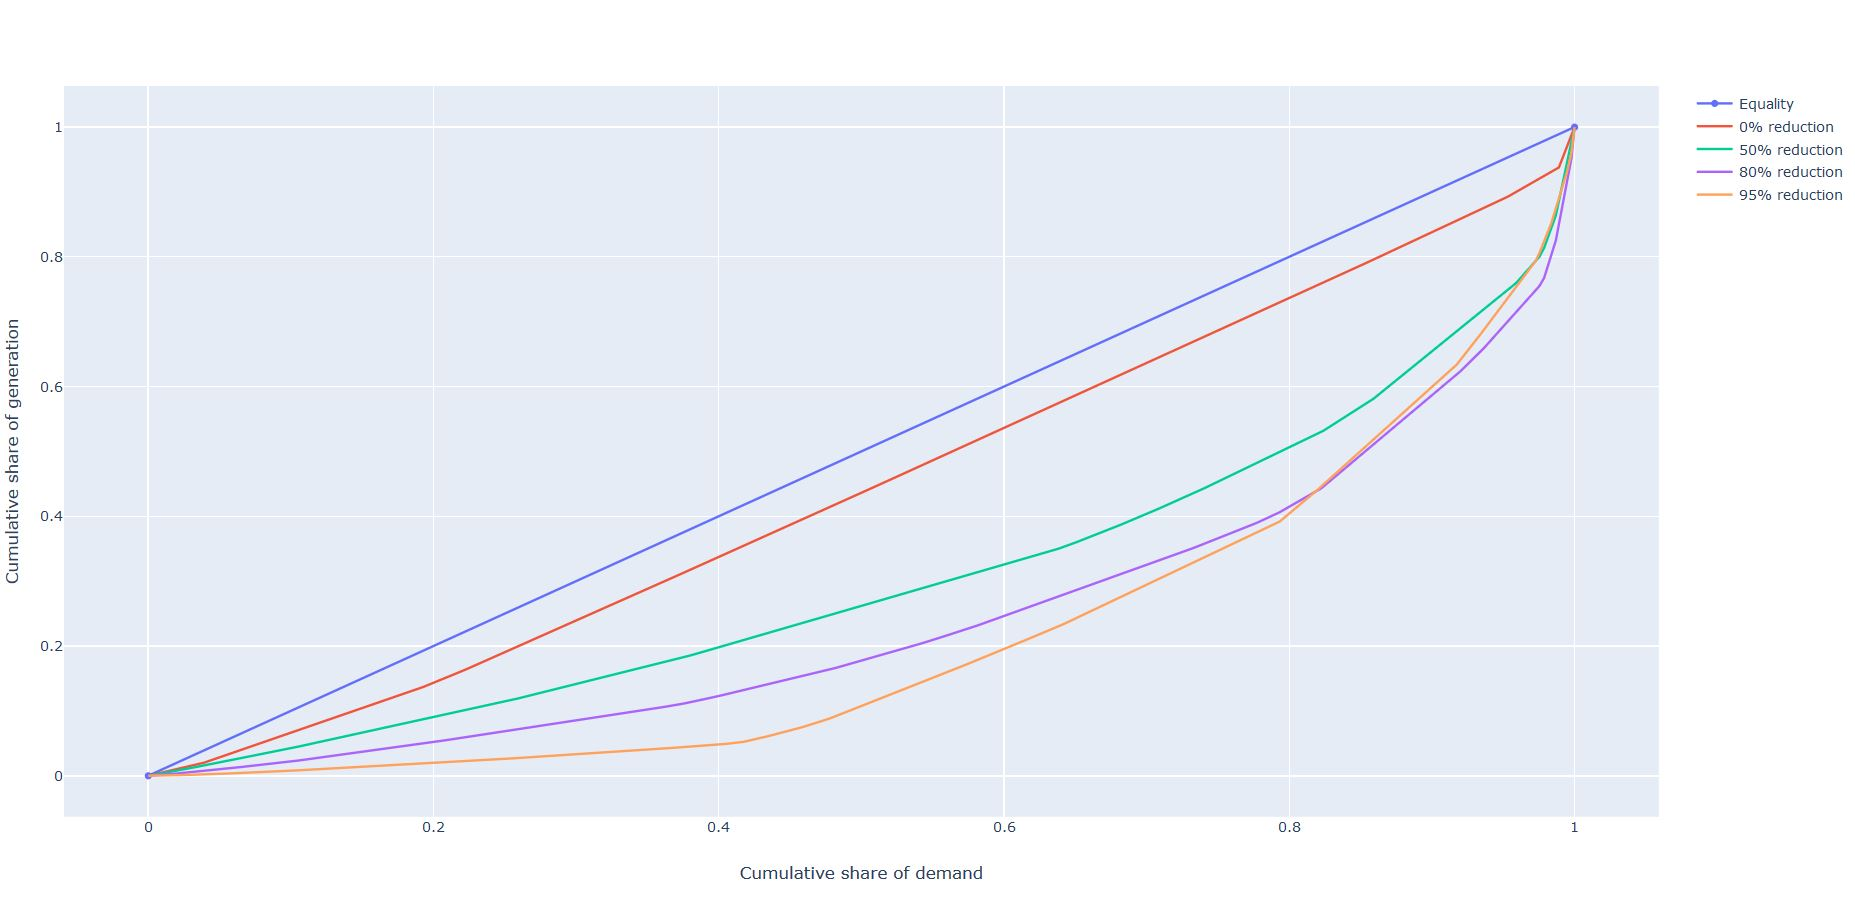
\includegraphics[width=1.\textwidth]{./Images/optimal_solutions_gini}
	\caption{Lorentz curves for the four optimal solutions \fxnote{Consider if this plot should stay}}
	\label{fig:Gini}
\end{figure}


\section{Implementation and utilization of parallel programming}
As the MGA approach described in section \ref{sec:Novel_MGA} requires a high number of similar optimizations to be performed only with slighly changed objective functions, it is possible to achieve a great performance boost, by utilizing parallel programming. 








